
\section{Task List}

\begin{tabular}{llrl}

    \toprule
    
    Task ID  & Task Description (Desc.)     & Due Date    & Deliverable       \\
    
    \midrule
    
    1        & Project Planning             & 14/02/2014  & Planning segment  \\
    1.1      & Mission Statement            & 07/02/2014  & Same as Desc.     \\
    1.2      & Mission Objectives           & 07/02/2014  & Project Goals     \\
    1.3      & Project Target               & 07/02/2014  & Project Scope     \\
    1.4      & Requirements                 & 07/02/2014  & Project Scope     \\
    1.5      & System Requirements          & 07/02/2014  & Same as Desc.     \\
    1.6      & User Requirements            & 07/02/2014  & Same as Desc.     \\
    1.7      & Transaction Requirements     & 07/02/2014  & Same as Desc.     \\
    
    \cmidrule(r){2-3}
    1.8      & Case Studies (CS)            & 14/07/2014  & Eval. of rival    \\
    1.8.1    & CS: Facebook                 & 14/07/2014  & Eval. of rival    \\
    1.8.2    & CS: 'GPG' and E-Mail         & 14/02/2014  & Eval. of rival    \\
    1.8.3    & CS: 'Tor'                    & 14/02/2014  & Eval. of rival    \\
    \cmidrule(r){2-3}
    
    1.9      & Required Data                & 14/02/2014  & Same as Desc.     \\
    1.10     & Risk Assessment              & 14/02/2014  & Same as Desc.     \\
    1.11     & Anticipated Software         & 14/02/2014  & Project Estimates \\
    1.12     & Anticipated Experiments      & 14/02/2014  & Project Estimates \\
    1.13     & Anticipated Documentation    & 14/02/2014  & Project Estimates \\
    1.14     & Methods of Evaluation        & 14/02/2014  & Same as Desc.     \\
    1.15     & User View                    & 14/02/2014  & Same as Desc.     \\
    1.16     & Gantt Chart                  & 14/02/2014  & Same as Desc.     \\
    1.17     & PERT Chart                   & 14/02/2014  & Same as Desc.     \\
    
    \midrule
    
    2        & Project Design               & 14/03/2014  & Design Segment    \\
    
    \cmidrule(r){2-3}
    2.1      & Research (Res.)              & 21/02/2014  & Research Segment  \\
    2.1.1    & Res: Database Languages      & 21/02/2014  & Same as Desc.     \\
    2.1.2    & Res: Programming Languages   & 21/02/2014  & Same as Desc.     \\
    2.1.3    & Res: Interfaces              & 21/02/2014  & Same as Desc.     \\
    \cmidrule(r){2-3}
    
    2.2      & Designs (Des.)               & 07/03/2014  & Design Segment    \\
    2.2.1    & Des: Databases               & 28/02/2014  & Same as Desc.     \\
    2.2.2    & Des: Class Interfaces        & 28/02/2014  & Same as Desc.     \\
    2.2.3    & Des: Protocol                & 28/02/2014  & Same as Desc.     \\
    2.2.4    & Des: Architecture            & 28/02/2014  & Same as Desc.     \\
    2.2.5    & Des: Sequence Diagrams       & 28/02/2014  & Same as Desc.     \\
    2.2.6    & Des: Data Flow Diagrams      & 28/02/2014  & Same as Desc.     \\
    2.2.7    & Des: Class Diagrams          & 28/02/2014  & Same as Desc.     \\
    2.2.8    & Des: Server-side Interfaces  & 28/02/2014  & Same as Desc.     \\
    2.2.9    & Des: Client-side Interfaces  & 28/02/2014  & Same as Desc.     \\
    2.2.10   & Des: Server-side Protocols   & 28/02/2014  & Same as Desc.     \\
    2.2.11   & Des: Client-side Protocols   & 28/02/2014  & Same as Desc.     \\
    2.2.12   & Des: Server-side Pseudo-code & 07/03/2014  & Same as Desc.     \\
    2.2.13   & Des: Client-side Pseudo-code & 07/03/2014  & Same as Desc.     \\
    \cmidrule(r){2-3}
    
    2.3      & Segment Review               & 10/03/2014  & Design Segment    \\
    2.3.1    & Evaluate Segment Quality     & 14/03/2014  & N/A               \\
    2.3.2    & Improve Segment              & 14/03/2014  & Design Segment    \\
    
    \midrule
    
    3        & Implementation stage (Imp.)  & 28/04/2014  & Imp. Segment      \\
    3        & Implementation stage (Imp.)  & 28/04/2014  & Imp. Segment      \\
    
    
    \midrule
    
    4        & Project Portfolio            & 09/05/2014  &  \\
    
    
    
    \bottomrule

\end{tabular}


\section{Gantt Chart}
\textit{gantt and pert chart, along with discussion of their value and
applicability}


\section{PERT Chart}


\section{System Boundary Diagram}
\textit{description of diagram, and why it is useful}
\begin{figure}[h]
    \centering
    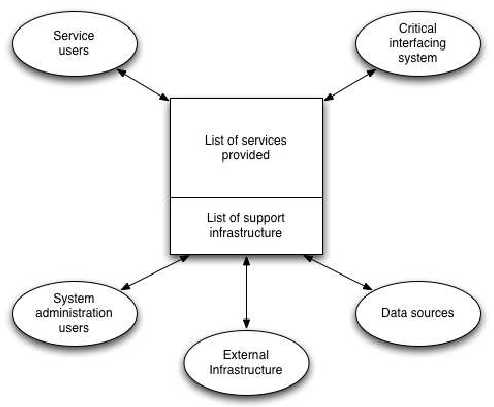
\includegraphics[width=0.7\textwidth]{images/requirements/system_boundary_diagram.png}
    \caption{System Boundary Diagram}
    \label{fig:sys_boundary_diag}
\end{figure}
